\documentclass[10pt]{article}
\usepackage[english]{babel}
\usepackage{lmodern}
\usepackage[T1]{fontenc}
\usepackage[protrusion=true,expansion=true]{microtype}
\usepackage{url}
\usepackage{graphicx}
\usepackage{float}
\graphicspath{ {./figures/} }
\hyphenation{Hirsch-muel-ler}



\begin{document}

\begin{titlepage}
	\begin{center}
		\vspace*{1.0cm}

    	{\fontsize{17}{16}\selectfont \textbf{Sea Wave Modelling and Prediction Based on Multisensor Fusion}}


		\vspace{1.0cm}
		Final Report of the Capstone Project

		\vspace{1.5cm}

		\textbf{Alexandre Ferreira}

				\vfill

		
\includegraphics[width=0.4\textwidth]{UPORTO_fundotransparente}

		\vfill



		Bachelor's Degree in Informatics and Computing Engineering

		\vspace{0.8cm}


		\textbf{Tutor at U.Porto}: Prof. Pedro Ribeiro\\
		\textbf{Company/Proposer Supervisor}: Prof. Eduardo Silva \\

\vspace{0.4cm}
		June 29, 2026

	\end{center}
\end{titlepage}

\thispagestyle{empty}
\clearpage

\begin{abstract}
This report presents an end-to-end ROS~2 pipeline for sea-surface reconstruction and wave-parameter estimation from a multi-sensor rig -- stereo cameras, laser altimeters, and a GNSS/INS navigation solution -- mounted on a support vessel. The central engineering challenge is stereo matching on the sea surface, which is low-texture, specular, and non-Lambertian: conditions that systematically break classical photometric methods. Six disparity-estimation backends -- three classical, three learned -- are systematically compared under identical pipeline conditions; the results show a clear and consistent quality gap between learned and classical architectures on this target, with the WAFT-Stereo backend achieving zero dropped frames in the downstream wave estimator. Two independent sea-state estimators are implemented and cross-validated without external ground truth: a temporal spectral estimator driven by a single laser altimeter and a spatial estimator derived from the georeferenced stereo point cloud. The two estimators agree on significant wave height ($H_s \approx 0.4$--$0.5$~m) and peak period ($T_p \approx 3.2$~s vs.\ $\approx$3.7~s) to within $\approx$10--13\%. This mutual agreement constitutes the primary validation of the pipeline's wave-parameter outputs in the absence of a wave buoy.
\end{abstract}
\thispagestyle{empty}
\clearpage

\thispagestyle{empty}
\tableofcontents

\clearpage

\section{Introduction}

\subsection{Context}

This internship is carried out within the scope of the SEAWINGS and AIRSHIP projects, initiatives aimed at developing innovative autonomous aerial platforms specifically designed to operate over maritime environments. The distinguishing feature of these platforms is their design as Wing-In-Ground (WIG) effect vehicles. These vehicles stand out for the operational requirement of flying at high speeds and extremely low altitudes, often only one or two metres above the water surface. This flight configuration takes advantage of the aerodynamic "ground effect" phenomenon, creating a cushion of air beneath the structure that drastically increases the vehicle's lift and energy efficiency.

\begin{figure}[h]
     \centering
          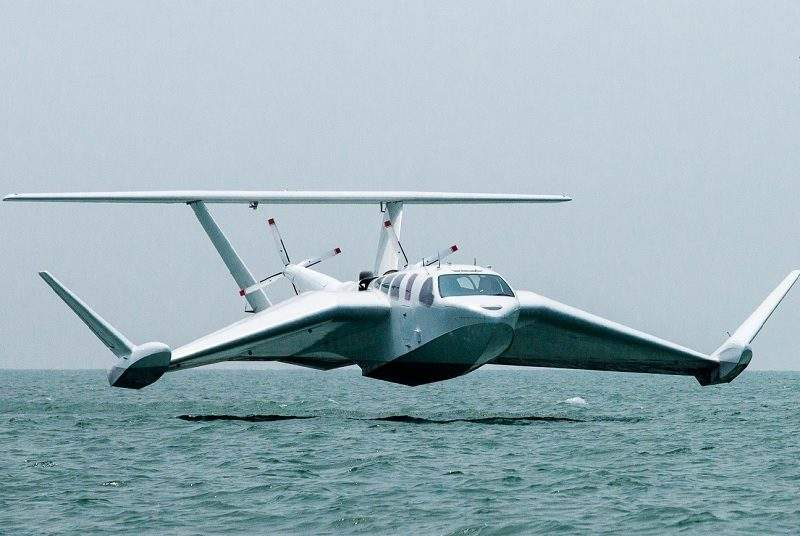
\includegraphics[width=0.7\textwidth]{../imagens/wig.jpg}
     \caption{Example of a vehicle operating under the Wing-In-Ground (WIG) effect principle.}
     \label{fig:wig_effect}
 \end{figure}

Because of this requirement for fast, low-altitude flight, one of the central and most critical challenges of these projects is accurate, real-time perception of the sea surface. In an environment where the margin for error is minimal and the fluid dynamics are unpredictable, timely detection of waves is not merely a matter of topographic mapping, but a fundamental safety requirement. The ability to "see" the water ahead of the vehicle ensures that the control systems can perform evasive manoeuvres or altitude adjustments, avoiding catastrophic collisions with the swell.

Ocean waves are a dynamic and periodic phenomenon, characterized mainly by their amplitude, direction and frequency. Correctly estimating the geometric and kinematic values of these parameters, as well as the ability to predict the short-term temporal and spatial propagation of waves, contributes significantly to the robustness of the control and trajectory-planning systems of these platforms under development.


\subsection{Related work}

\textbf{Sea-state sensing.}
The canonical instrument for sea-state monitoring is the moored wave buoy, which records heave acceleration and integrates it to recover sea-surface elevation. Buoys yield accurate spectral and directional estimates but require fixed deployment infrastructure and return only a single spatial point. X-band marine radar~\cite{rs9121261} is the established ship-mounted alternative: backscatter images of the sea surface encode the directional wave spectrum and can be processed in near-real-time, but the hardware is heavy, power-hungry, and designed for vessels far larger than the WIG platforms targeted here. Single-point laser and ultrasonic altimeters~\cite{toa2020ultrasonic} are lightweight and compact but similarly provide no spatial coverage. The WIG application requires a sensing solution that is lightweight, operates from a moving low-altitude platform, and reconstructs the sea surface geometrically ahead of the vehicle -- a combination that none of these established modalities addresses directly.

\textbf{Stereo reconstruction of the sea surface.}
Non-contact stereo wave measurement was first demonstrated at oceanographic scale by Benetazzo~\cite{benetazzo2006offshore} and subsequently productised in the open-source WASS pipeline~\cite{bergamasco2017wass}, which achieved sub-centimetre reconstruction accuracy from a near-fixed, near-vertical platform using Hirschmüller's semi-global matching (SGM)~\cite{hirschmuller2008stereo}. Later work targeting the sea surface's photometric adversity -- low texture over large areas and specular non-Lambertian reflections that violate brightness constancy -- includes GPU-accelerated feature-based stereo on ship-mounted rigs~\cite{app12157447}, stereo for maritime object localisation~\cite{jmse12010197}, and thermal stereo~\cite{li2025thermal}, which sidesteps visible-spectrum specularity by imaging in the long-wave infrared at the cost of a more specialised and expensive sensor pair.

\textbf{Stereo-matching architectures.}
Classical SGM~\cite{hirschmuller2008stereo} applies global path-wise smoothness regularisation over the disparity image, allowing it to recover coherent depth over mildly textureless regions -- making it the strongest classical baseline available without training data. Learned architectures have consistently outperformed it on standard benchmarks: HITNet~\cite{DBLP:journals/corr/abs-2007-12140} propagates disparity hypotheses over a hierarchical tile pyramid without building a full 4D cost volume, enabling real-time inference; RAFT-Stereo~\cite{DBLP:journals/corr/abs-2109-07547} applies iterative GRU updates over a multi-level correlation volume for high accuracy at higher latency; WAFT-Stereo~\cite{wang2026waftstereowarpingalonefieldtransforms} replaces cost-volume lookups with warping-alone field transforms, reaching state-of-the-art benchmark performance at latency comparable to RAFT-Stereo.

\textbf{Wave-parameter estimation and platform motion.}
Spectral wave parameters -- significant wave height $H_s = 4\sqrt{m_0}$, peak period $T_p$, and spectral mean periods $T_{m01}$/$T_{m02}$ -- are defined against the directional wave spectrum, whose canonical empirical forms are the Pierson--Moskowitz spectrum for fully-developed seas~\cite{pierson1964spectral} and the JONSWAP spectrum for fetch-limited wind-sea growth~\cite{Hasselmann1973}. Altimetric estimation from a moving platform introduces the encounter-frequency effect: a platform travelling through the wave field at speed $U$ measures an encounter period rather than the true period, the two being related via the deep-water dispersion relation and the relative heading between platform and waves~\cite{dean1991water}. Ichikawa et al.~\cite{ichikawa2024seasurface} demonstrated this correction explicitly for a UAV-mounted nadir LiDAR altimeter -- the closest published configuration to the one used in this project -- and quantified the resulting period shift.

\textbf{Short-term wave forecasting.}
Deterministic wave forecasting from reconstructed wave fields propagates the phase-resolved spectrum forward in time using linear wave theory~\cite{naaijen2010real,qi2018predictable}, with the forecast horizon set by the predictable zone of the measurement. Data-driven methods using recurrent networks~\cite{hochreiter1997long} and attention-based architectures~\cite{vaswani2017attention} have been applied to longer-horizon statistical forecasting. This work focuses on parameter \emph{estimation} -- a prerequisite for any forecasting stage -- and treats forecasting as a descoped but natural next step (Section~\ref{sec:future}).


\subsection{Objectives and expected results}

O principal objetivo do estágio é o estudo, desenvolvimento e validação de abordagens de perceção e modelização de ondas oceânicas, baseadas em arquiteturas de fusão multissensoria adaptadas às limitações e requisitos operacionais de plataformas aéreas autónomas de Efeito de Solo (WIG). 

\subsection{Report structure}

The remainder of this report is organized as follows. Section~2 describes the methodology followed during the internship, the stakeholders involved, and the timeline of activities. Section~3 covers the solution itself: the functional and non-functional requirements, the pipeline architecture and the technical difficulties encountered (with particular emphasis on the search for a stereo-matching backend that works on the sea surface), the solution from a user's perspective, and its validation through cross-checks between independent sensing modalities and against an independent navigation reference. Section~4 concludes with the results achieved against the original objectives, the lessons learned, identified future work, and the project's relation to the Sustainable Development Goals.


\section{Methodology}

The work followed an iterative, data-first engineering process rather than a fixed up-front design. Each milestone began by inspecting real recorded data (topic schemas, physical units, coordinate frames and clock domains) before any code was written, and ended with a verification step against that same data once a node or fix was in place. This loop of characterizing the raw data, implementing against it, and then re-verifying the result on that same data was applied consistently across the project: position and orientation corrections on the pointcloud, altimeter data cleaning and the disparity-backend search were all driven by first characterizing the raw sensor output and only then developing the code, rather than relying only on vendor documentation or conventions.

Progress was tracked through screenshots, plots and short video clips of the pipeline's output, which were shared with the supervisors for feedback. The project was developed in a single Git repository, with a main branch for stable code and feature branches for new nodes or fixes. Each commit was accompanied by a descriptive message, and the commit history was used to track progress and decisions made during development.

The technology stack was: ROS~2 Humble with the Zenoh middleware implementation, Python (\texttt{rclpy}), OpenCV (classical and CUDA-accelerated stereo matching), PyTorch and ONNX Runtime (learned stereo-matching backends), and Git~\cite{github} for version control. No dedicated project-management tooling was used; given the single-person, single-supervisor nature of the internship, coordination with supervisors was handled through periodic meetings rather than a formal sprint/ticket process.


\subsection{Stakeholders, roles and responsibilities}

This was an individual internship, with the following roles:

\begin{itemize}
	\item \textbf{Alexandre Ferreira} (student): bibliographic research, pipeline design and implementation, data analysis, validation, and reporting.
	
	\item \textbf{Prof. Pedro Ribeiro} (tutor, U.Porto): responsible for academic supervision and periodic follow-up on project direction and scope.

	\item \textbf{Prof. Eduardo Silva} (company/proposer supervisor): supervision on behalf of INESC~TEC.
	
	\item \textbf{Guilherme Amaral, Jos\'{e} Carlos Fernandes, and Maksym Lysak} (INESC~TEC, SEAWINGS/AIRSHIP team): provided day-to-day technical support and held regular working meetings throughout the internship.
\end{itemize}


\subsection{Activities carried out}

The internship followed the five phases of the original work plan (literature review, sensor characterization, estimation-algorithm development, wave modelling/prediction, validation and documentation). The work is summarized as an ordered sequence of milestones in Table~\ref{tab:activities}.

\begin{table}[H]
	\centering
	\caption{Project timeline.}
	\label{tab:activities}
	\small
	\begin{tabular}{@{}cp{0.82\textwidth}@{}}
		\textbf{Week} & \textbf{Milestone} \\
		\hline
		1-2 & Literature review for sensor selection and wave modelling. ROS~2 setup. \\
		3 & Incorporated feedback from the team on the literature review. \\
		4 & Sensor-fusion literature review. \\
		5 & Began hands-on ROS~2 learning and early disparity/point-cloud experiments on a provided drone-flight dataset. \\
		6 & Early disparity/point-cloud attempts had limited success; switched to validating the pipeline on a simpler static-camera case first, with collected camera calibration data. \\
		7-8 & Tested multiple disparity backends and tuned their parameters. Good results on the calibration dataset, which was recorded inside the lab. \\
		9 & Additional disparity backends added and compared (classical and machine-learning based). Only decent results achieved were on HitNet and RAFT-Stereo.\\
		10 & Single command pipeline start; Pointcloud roll/orientation correction via horizon line detection. \\
		11 & New disparity backend tested with better results (WAFT-Stereo);The team supplied the calibrated navigation bags, unblocking pose work. \\
		12 & Rig URDF geometry obtained; WAFT-Stereo backend integrated in the pipelineand tuned ($\sim$150\,ms/frame), outperforming HITNet. \\
		12--13 & Altimeter wave-estimation node creation and tuning (band-limiting fix); point-cloud bad-frame gate added. \\
		13 & Point-cloud wave estimator reconciled with the altimeter estimator (range filter + median aggregation). \\
		14 & Doppler/encounter-frequency correction resolved the wave period disagreement between estimators. \\
		15 & Final disparity-backend comparison campaign (six backends, tuned vs.\ default); validation and report writing. \\
	\end{tabular}
\end{table}

As anticipated in the project plan, the search for a disparity-estimation backend that performs adequately on the sea surface was not a single milestone but a recurring thread throughout the project, beginning with the first early experiments and still being actively revisited in the final comparison campaign.


\section{Solution development}

\subsection{Requirements}

\textbf{Functional requirements:}
\begin{itemize}
	\item Reconstruct a 3D point cloud of the sea surface in real time (per recorded frame).
	\item Georeference that point cloud by fusing it with an independent navigation/pose solution.
	\item Estimate sea-state parameters (significant wave height ($H_s$), peak period ($T_p$) and, where feasible, propagation direction).
	\item Validate the point cloud by cross-checking the sea-state parameters against an independent sensing modality.
\end{itemize}

\textbf{Non-functional requirements:}
\begin{itemize}
	\item The system must operate with minimum latency, with a target of $\leq$\, 200ms from frame capture to point-cloud output.
	\item The system must be reliable and robust to the specific challenges of the sea surface (low texture, specularity) and to the operational conditions of a moving platform (vibrations, rolling/pitching, changing lighting conditions).
	\item The system must be modular and maintainable, allowing for easy integration of new sensors or algorithms, and for future upgrades to the stereo-matching backend or wave-estimation methods.
\end{itemize}

\textbf{Constraints:}
\begin{itemize}
	\item \begin{sloppypar}The system must operate on a single embedded edge-AI module (NVIDIA Jetson Orin Nano-class, 8~GB shared memory), which imposes strict constraints on the GPU budget available for disparity estimation.\end{sloppypar}
	\item Development and testing were limited to the hardware and tooling available: a single development workstation, the existing test structure, with limited scope to alter the physical setup, in order to mimic the conditions of the final deployment.
	\item Validation depended on recorded datasets, as due to time constraints and meteorological conditions, no further test campaigns could be run in order to gather data under different or rougher sea states and test the pipeline live on the vessel.
\end{itemize}


\subsection{Architecture and technologies}

\label{sec:architecture}

\textbf{Pipeline overview.} The system is a chain of ROS~2 nodes operating on a calibrated stereo pair, a navigation/INS solution, and a set of laser altimeters. A rectification node undistorts and rectifies the raw stereo images and publishes the corresponding camera calibration. Its output feeds a disparity-estimation node (interchangeable between six backends, discussed below), whose disparity map is reprojected into a coloured 3D point cloud. In parallel, a pose-broadcasting node consumes the navigation solution and publishes the platform's pose and a map~$\leftrightarrow$~body transform, which georeferences the point cloud and is also used by an altimeter-publishing node to place the laser-altimeter readings in the same frame. Two further nodes consume this georeferenced data to estimate sea-state parameters independently: one analyses the temporal signal from a single altimeter, the other analyses the spatial geometry of the stereo point cloud. Figure~\ref{fig:pipeline-architecture} summarises the node graph and the topics connecting each stage.

\begin{figure}[H]
	\centering
	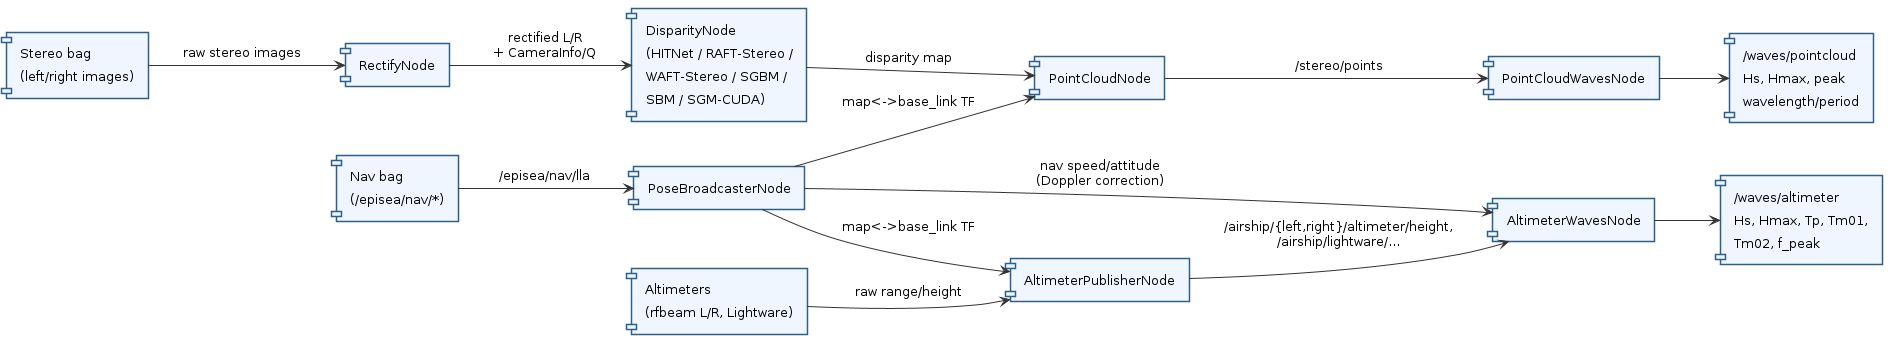
\includegraphics[width=\textwidth]{pipeline_architecture}
	\caption{Pipeline architecture: ROS~2 nodes and the topics connecting them.}
	\label{fig:pipeline-architecture}
\end{figure}

\begin{figure}[H]
	\centering
	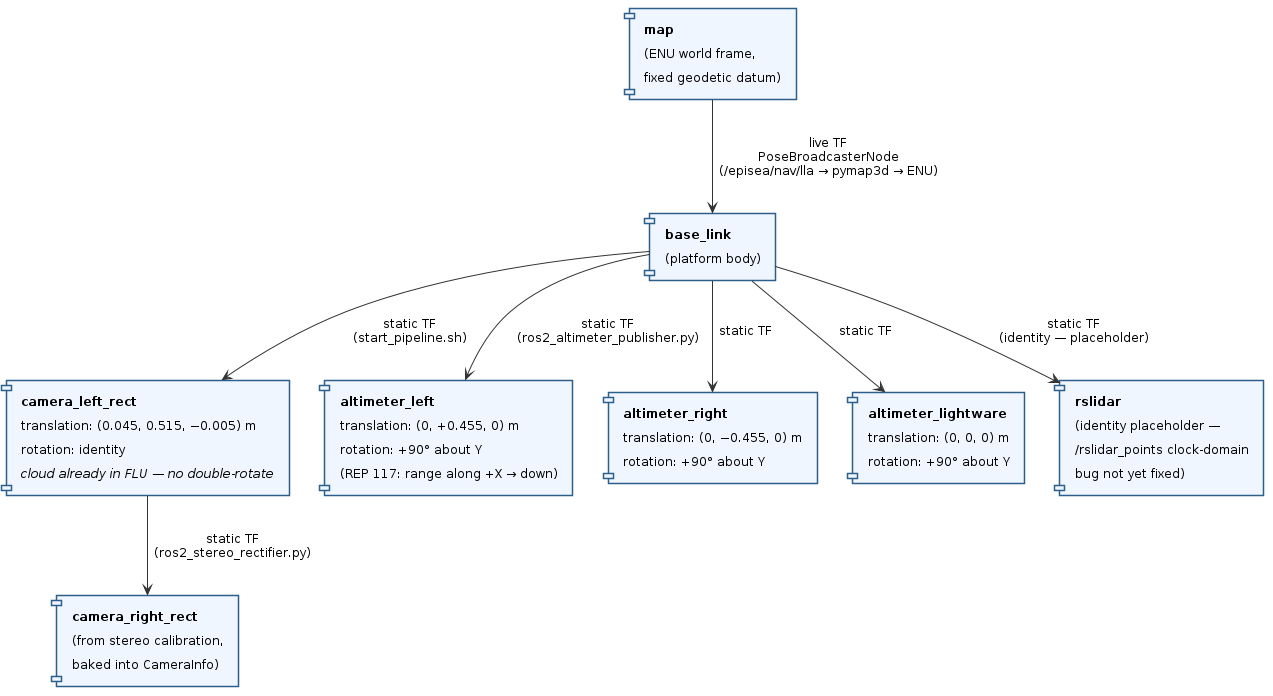
\includegraphics[width=0.85\textwidth]{diagrams/tf_frame_tree}
	\caption{Sensor frame tree. Static transforms are wired at startup; the map~$\leftrightarrow$~base\_link transform is published live by the pose-broadcasting node. The \texttt{rslidar} transform remains an identity placeholder pending resolution of a clock-domain timestamp mismatch in the lidar recording.}
	\label{fig:tf-frame-tree}
\end{figure}

\subsection*{Disparity-estimation methods and comparison}

\begin{figure}[H]
	\centering
	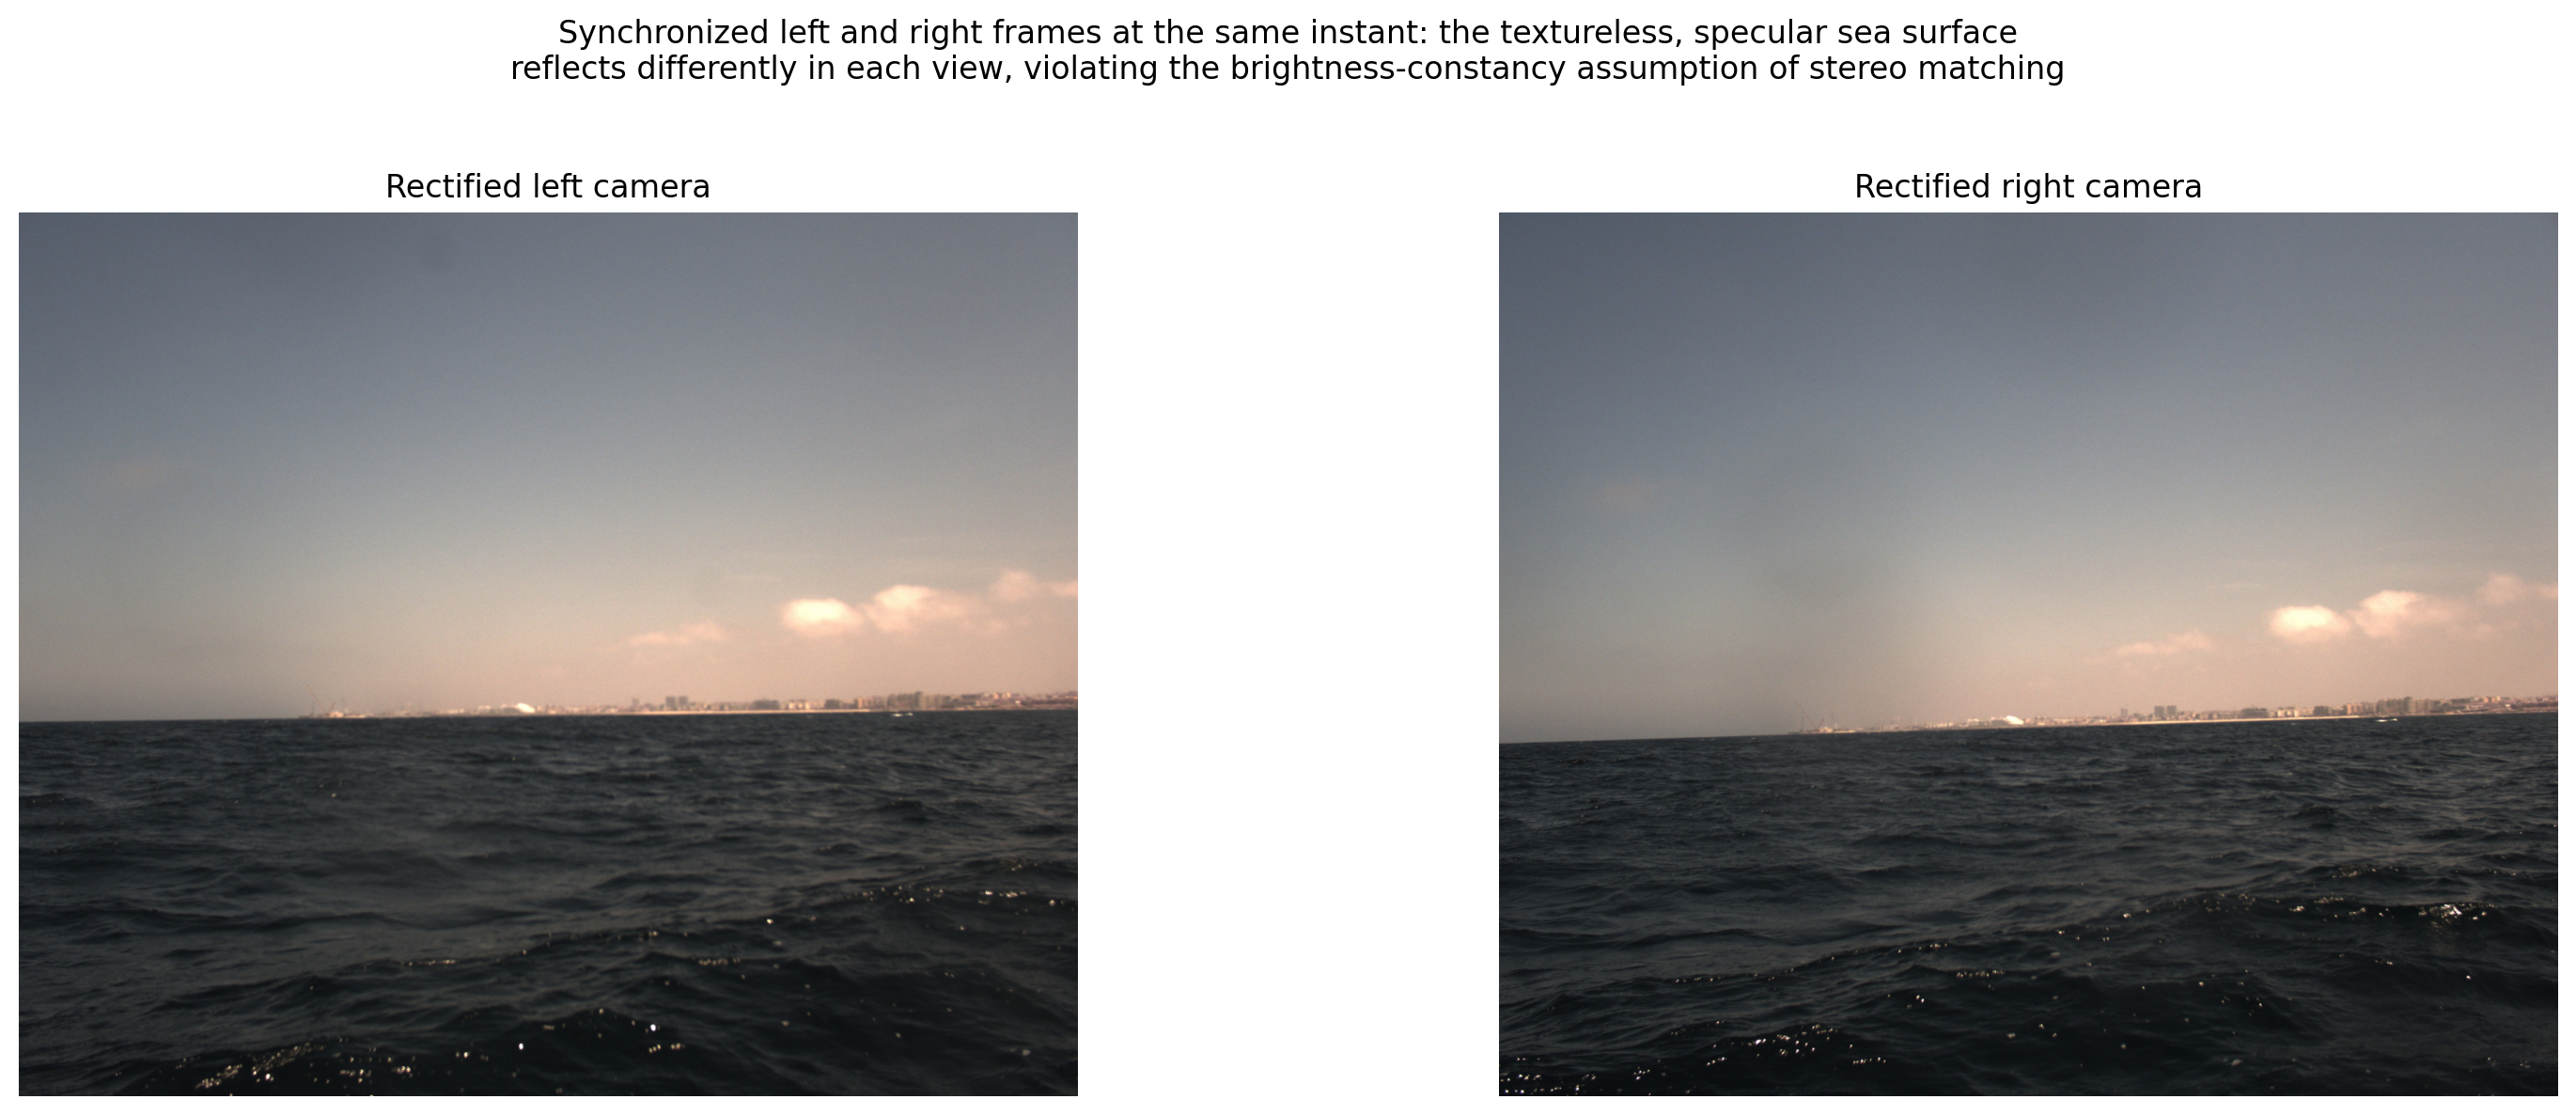
\includegraphics[width=0.85\textwidth]{original_camera_footage}
	\caption{Typical left-camera frame from the stereo bag. The sea surface is largely textureless with specular highlights, making it an adversarial target for photometric stereo matching.}
	\label{fig:raw-camera}
\end{figure}

\begin{figure}[H]
	\centering
	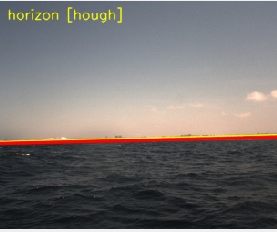
\includegraphics[width=0.85\textwidth]{horizon_detection}
	\caption{Sky/horizon masking applied by the shared pre-processing stage. Pixels above the detected horizon line (shown in red) are excluded from disparity estimation and point-cloud reconstruction, preventing sky matches from corrupting the sea-surface output.}
	\label{fig:horizon-detection}
\end{figure}

The sea surface is a uniquely adversarial target for stereo matching: it is low-texture over large areas, and its specular, non-Lambertian reflections change with viewpoint and violate the brightness-constancy assumption that local photometric matching relies on. The combination of ambiguous matches in textureless regions, plus systematically wrong matches under specular highlights breaks classical block-matching stereo, and is well documented in stereo-vision work specifically targeting maritime/wave surfaces~\cite{app12157447,jmse12010197,li2025thermal}. Identifying a backend that copes with this was the central engineering problem of the project, more so than any individual integration bug, and is treated as the main result of the Architecture work.

Six interchangeable disparity-estimation backends were implemented and evaluated, sharing the same input/output contract (rectified stereo pair in, scaled disparity and packed point-cloud-ready output out, plus shared sky/horizon masking) so that they are drop-in replacements for one another and a fair comparison is possible without touching the rest of the pipeline:

\begin{itemize}
	\item \textbf{Classical, no training data required:} block matching (StereoBM, fastest, weakest on low-texture targets), semi-global matching (StereoSGBM, using Hirschmüller's global smoothness formulation~\cite{hirschmuller2008stereo}, the strongest classical option but slower), and a GPU-accelerated semi-global matcher (\texttt{cv2.\allowbreak{}cuda.\allowbreak{}StereoSGM}, SGM-style quality targeting GPU-class throughput).
	\item \textbf{Machine learning-based:} HITNet~\cite{DBLP:journals/corr/abs-2007-12140} (a hierarchical network that propagates disparity hypotheses and confidences across a tile pyramid rather than building an explicit cost volume, enabling real-time inference), RAFT-Stereo~\cite{DBLP:journals/corr/abs-2109-07547} (tuned via mixed precision and a reduced iteration count to fit the VRAM budget), and WAFT-Stereo~\cite{wang2026waftstereowarpingalonefieldtransforms} (a warping-alone field-transform architecture, state-of-the-art on standard stereo benchmarks at publication time; the smallest of its three published checkpoint sizes was used to fit the available VRAM).
\end{itemize}

\subsubsection*{Comparison methodology and results}

All six backends were run, one at a time, against the same $\sim$90-second recorded segment (after a fixed warm-up period), in an otherwise identical pipeline (navigation playback, pose broadcaster, rectifier, the disparity backend under test, point-cloud reconstruction, and the point-cloud wave estimator). Four metrics were recorded per backend: a photometric-consistency error on the disparity map (lower is better), the fraction of pixels with a valid disparity estimate, end-to-end latency, and as an end-to-end, application-level quality signal whether and how reliably the resulting point cloud was usable by the downstream wave estimator (its dropped-frame/good-frame ratio and the wave-height estimate it produced). The three classical backends were evaluated twice: with their library default parameters, and after a manual tuning pass confirmed on the full capture. Table~\ref{tab:disparity-comparison} reports the results.

\begin{table}[H]
	\centering
	\caption{Disparity-backend comparison on a fixed $\sim$90\,s recorded segment.}
	\label{tab:disparity-comparison}
	\small
	\resizebox{\textwidth}{!}{%
	\begin{tabular}{l c c c c c}
		\textbf{Backend} & \textbf{Photo.\ err.} & \textbf{Valid \%} & \textbf{Latency (ms, med/p90)} & \textbf{PC bad:good} & \textbf{PC $H_s$} \\
		\hline
		StereoBM, default      & n/a   & 0.0\%  & 9.4 / 10.9   & n/a (always empty) & n/a \\
		StereoBM, tuned        & 14.06 & 19.2\% & 8.7 / 10.1   & 3.7 & 0.97~m \\
		StereoSGBM, default    & 12.49 & 23.8\% & 43.9 / 53.0  & 2.2 & 0.91~m \\
		StereoSGBM, tuned      & 12.50 & 23.8\% & 40.3 / 45.9  & 1.0 & 0.90~m \\
		SGM-CUDA, default      & 13.22 & 7.1\%  & 10.1 / 11.2  & n/a (always empty) & n/a \\
		SGM-CUDA, tuned        & 12.92 & 17.0\% & 8.6 / 9.8    & n/a (always empty) & n/a \\
		HITNet                  & 14.27 & 35.8\% & 37.3 / 40.0  & 0.20 & 0.79~m \\
		RAFT-Stereo             & 12.90 & 33.7\% & 115.0 / 162.2 & 0.07 & 0.50~m \\
		WAFT-Stereo             & 12.92 & 36.0\% & 114.2 / 160.6 & 0.00 & 0.29~m \\
	\end{tabular}}
\end{table}

\begin{figure}[H]
	\centering
	\begin{minipage}[t]{0.48\textwidth}
		\centering
		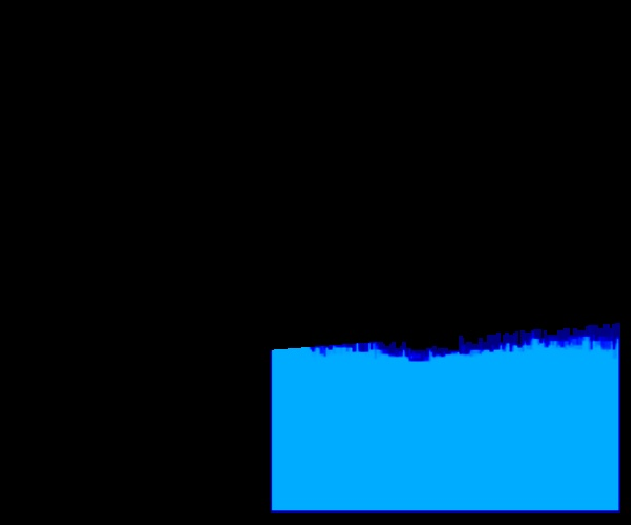
\includegraphics[width=\textwidth]{sbm_disparity}
	\end{minipage}\hfill
	\begin{minipage}[t]{0.48\textwidth}
		\centering
		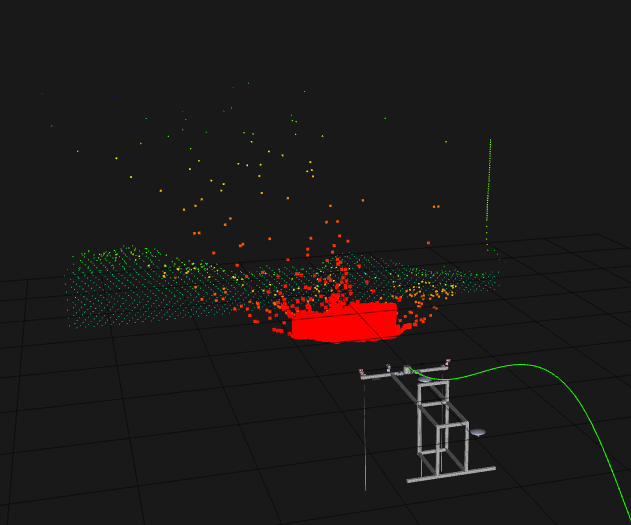
\includegraphics[width=\textwidth]{sbm_pc}
	\end{minipage}
	\caption{StereoBM (tuned): disparity map (left) and resulting point cloud (right). Large invalid regions reflect block matching's inability to find reliable matches on the textureless sea surface; the point cloud is sparse and noisy.}
	\label{fig:sbm-result}
\end{figure}

\begin{figure}[H]
	\centering
	\begin{minipage}[t]{0.48\textwidth}
		\centering
		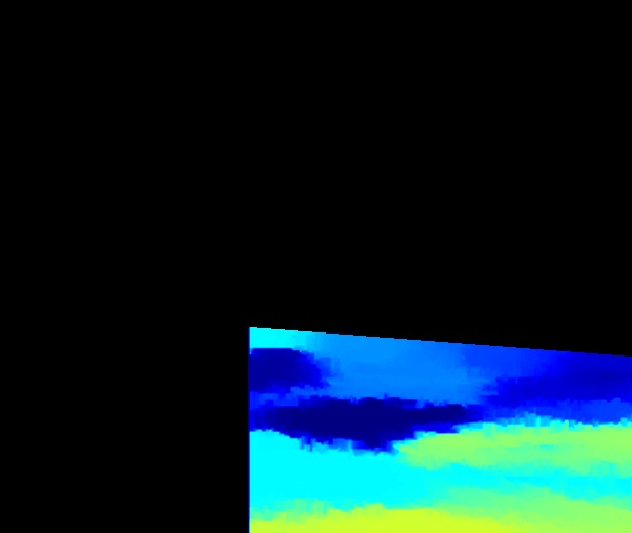
\includegraphics[width=\textwidth]{sgbm_disparity}
	\end{minipage}\hfill
	\begin{minipage}[t]{0.48\textwidth}
		\centering
		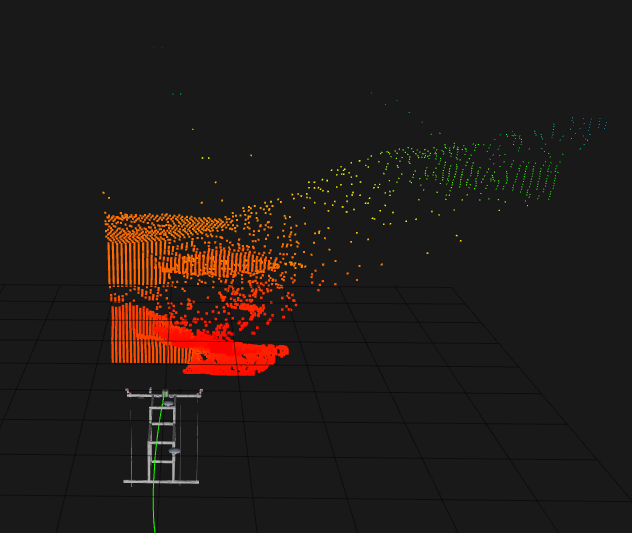
\includegraphics[width=\textwidth]{sgbm_pointcloud}
	\end{minipage}
	\caption{StereoSGBM (tuned): disparity map (left) and resulting point cloud (right). The global smoothness regularisation recovers more surface coverage than StereoBM, producing a denser cloud, though disparity failures remain frequent over specular patches.}
	\label{fig:sgbm-result}
\end{figure}

\begin{figure}[H]
	\centering
	\begin{minipage}[t]{0.48\textwidth}
		\centering
		
\includegraphics[width=\textwidth]{sgm_cuda_disparity}
	\end{minipage}\hfill
	\begin{minipage}[t]{0.48\textwidth}
		\centering
		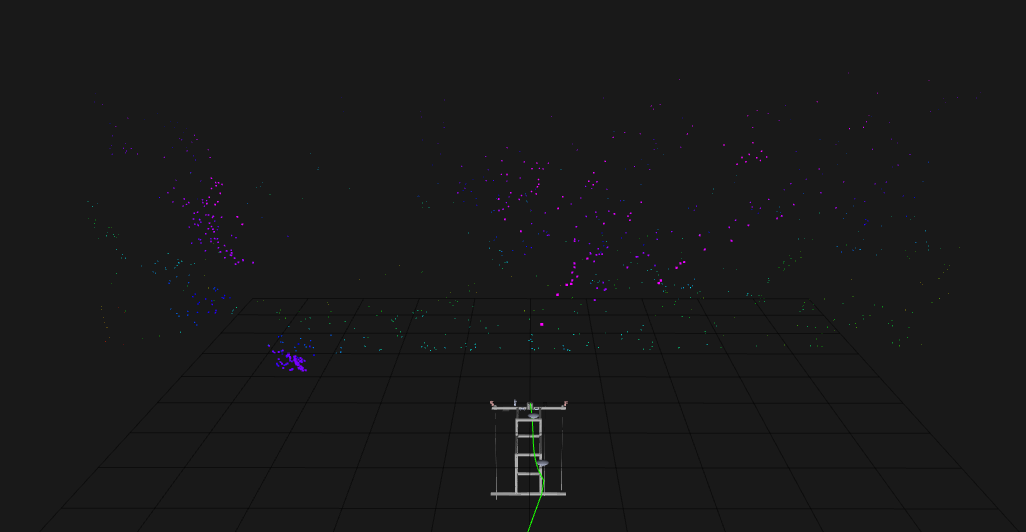
\includegraphics[width=\textwidth]{sgm_pc}
	\end{minipage}
	\caption{SGM-CUDA (tuned): disparity map (left) and resulting point cloud (right). GPU acceleration reduces latency relative to StereoSGBM but the absence of left--right consistency checking leaves the point cloud too sparse for the wave estimator to fit a surface.}
	\label{fig:sgm-cuda-result}
\end{figure}

\begin{figure}[H]
	\centering
	\begin{minipage}[t]{0.48\textwidth}
		\centering
		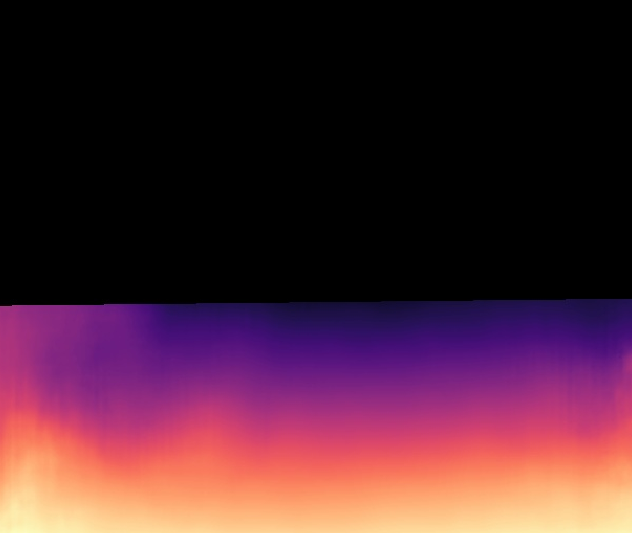
\includegraphics[width=\textwidth]{hitnet_disparity}
	\end{minipage}\hfill
	\begin{minipage}[t]{0.48\textwidth}
		\centering
		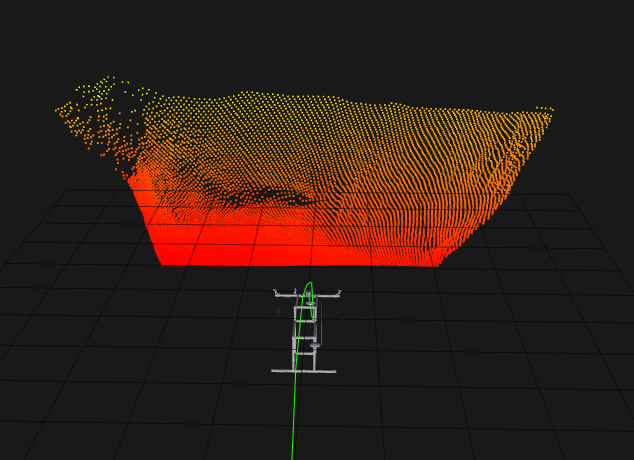
\includegraphics[width=\textwidth]{hitnet_pc}
	\end{minipage}
	\caption{HITNet: disparity map (left) and resulting point cloud (right). The learned backbone recovers substantially more valid disparity over textureless and specular areas, yielding a dense and well-structured sea-surface point cloud.}
	\label{fig:hitnet-result}
\end{figure}

\begin{figure}[H]
	\centering
	\begin{minipage}[t]{0.48\textwidth}
		\centering
		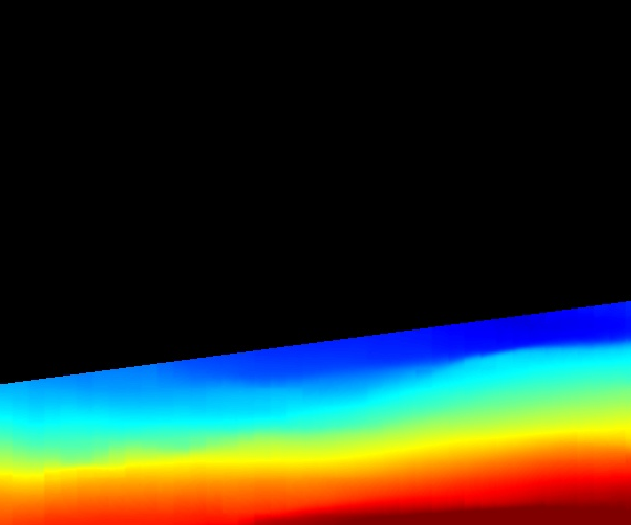
\includegraphics[width=\textwidth]{raft_disparity}
	\end{minipage}\hfill
	\begin{minipage}[t]{0.48\textwidth}
		\centering
		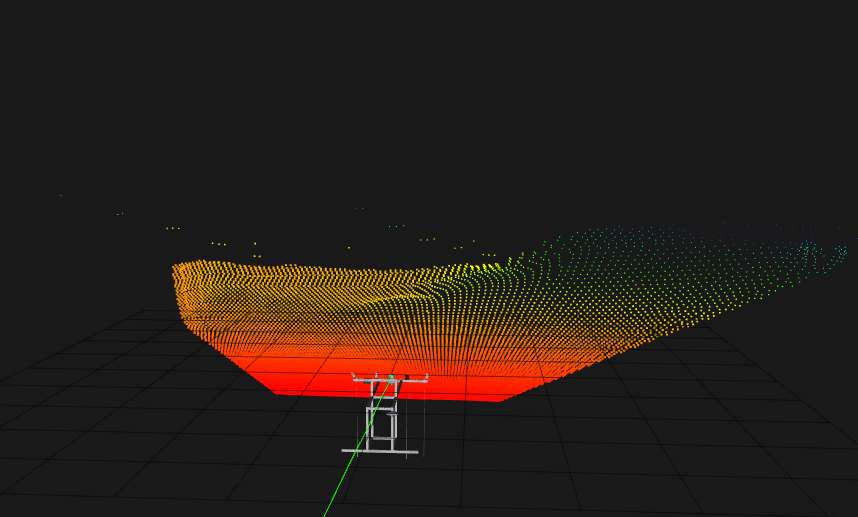
\includegraphics[width=\textwidth]{raft_pc}
	\end{minipage}
	\caption{RAFT-Stereo: disparity map (left) and resulting point cloud (right). The iterative correlation-volume approach handles the low-texture sea surface well, with a low bad-frame rate and a dense cloud, at the cost of higher latency than HITNet.}
	\label{fig:raft-result}
\end{figure}

\begin{figure}[H]
	\centering
	\begin{minipage}[t]{0.48\textwidth}
		\centering
		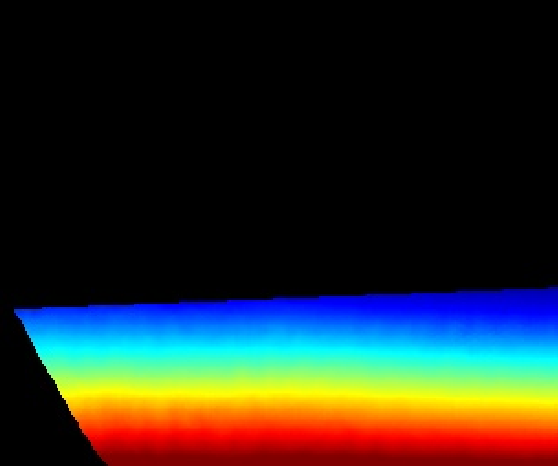
\includegraphics[width=\textwidth]{waft_disparity}
	\end{minipage}\hfill
	\begin{minipage}[t]{0.48\textwidth}
		\centering
		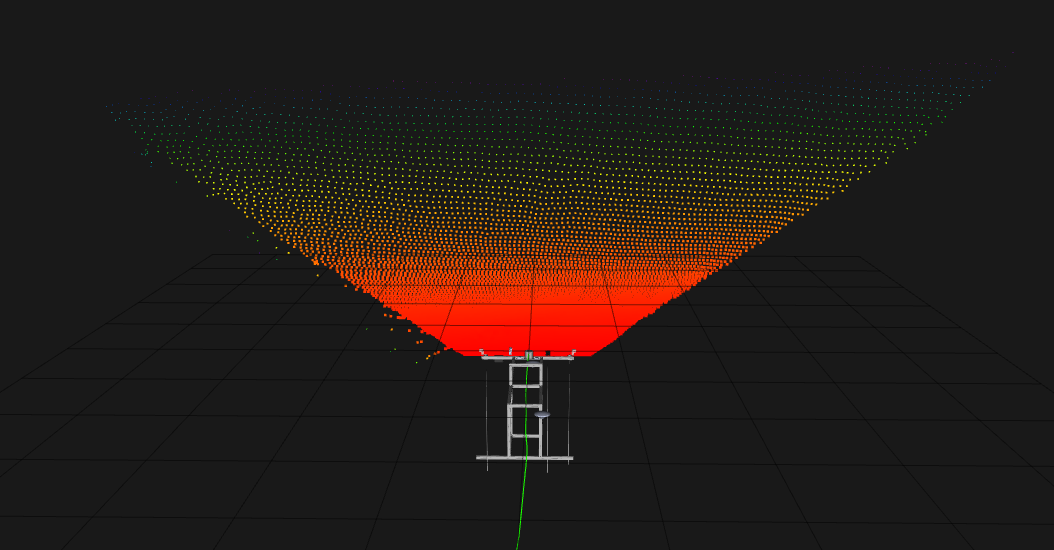
\includegraphics[width=\textwidth]{waft_pc}
	\end{minipage}
	\caption{WAFT-Stereo: disparity map (left) and resulting point cloud (right). The warping-alone field-transform architecture achieves zero dropped frames over the evaluation segment and produces the $H_s$ closest to the altimeter cross-validation reference, at latency comparable to RAFT-Stereo.}
	\label{fig:waft-result}
\end{figure}

\emph{PC bad:good} is the ratio of disparity-failure frames dropped by the point-cloud wave estimator's per-frame quality gate to good frames retained, measured over the most recent reporting window (not a cumulative 0--1 fraction); \emph{PC $H_s$} is the significant wave height the point-cloud estimator produced from the surviving frames. ``n/a (always empty)'' means the point cloud never had enough valid disparity to support a single sea-surface plane fit during the whole capture, so the wave estimator never produced a value at all.

\textbf{Reading the comparison.} Photometric error is fairly flat ($\approx$12.5--14.3) across every backend that produces any valid disparity at all: it mainly distinguishes ``works at all'' from ``does not'', rather than separating quality between working backends. The point-cloud bad:good ratio and resulting $H_s$ are more discriminating: StereoSGBM and tuned StereoBM are the only classical configurations that ever produced a usable point cloud, and even then with a substantially worse bad:good ratio than any of the three learned backends. Tuning matters more between the classical methods themselves than between the classical and learned families: StereoBM's apparent total failure under default parameters (0\% valid, no point cloud at all) turned out to be mostly a parameter-choice artifact, once tuned it reaches 19.2\% valid and does produce a (low-quality) point cloud, so the fair claim is that StereoBM's library defaults do not work on this scene, not that block matching cannot work on water at all. StereoSGBM barely moved between default and tuned parameters, indicating its defaults were already close to its ceiling for this scene. SGM-CUDA improved substantially with tuning (7.1\%$\to$17.0\% valid) but never reached the point where the wave estimator could fit a surface even once; this is plausibly explained by the GPU binding used here exposing no left--right consistency control equivalent to StereoSGBM's, rather than a fundamental SGM limitation. Even after tuning, all three classical methods remain clearly behind the three learned backends on the metric that matters for this application: whether a usable point cloud is produced at all, and how reliably.

Among the learned backends, HITNet has the lowest latency (37~ms) and a markedly better bad:good ratio than the classical methods, consistent with its selection as the pipeline's default. RAFT-Stereo and WAFT-Stereo show near-identical photometric quality and valid fraction (expected, given their closely related architectures), but WAFT-Stereo achieves a better bad:good ratio (zero dropped frames across the entire evaluation segment) and is also the backend whose $H_s$ estimate is most interpretable: with no bad frames contaminating the buffer, its 0.29~m figure is not inflated by residual disparity failures, unlike HITNet (0.79~m, bad:good 0.20) and RAFT-Stereo (0.50~m, bad:good 0.07), which still pass a fraction of marginal frames through the quality gate. The remaining gap between WAFT-Stereo's 0.29~m and the altimeter's time-varying range of $\approx$0.4--0.6~m is consistent with two known geometric effects: the 40~m near-field patch spans only two to three wavelengths, which undersamples the wave field spatially, and the plane fit over an oblique patch partly absorbs long-wavelength elevation as surface tilt rather than residual variance, as quantified in Section~\ref{sec:validation}. Furthermore, the altimeter's 0.4--0.6~m is itself a range over the full recording, not a fixed reference; during the calmer intervals of the $\sim$90~s comparison window the altimeter's own instantaneous estimate falls toward its lower end, narrowing the residual gap further. Both RAFT-Stereo and WAFT-Stereo measured $\approx$114--115~ms median latency in this full-pipeline setting, above the sub-100~ms figure quoted for RAFT-Stereo-style architectures in isolation; this reflects GPU/CPU contention with the rest of the running pipeline (rectification, point-cloud construction, wave estimation) rather than a clean per-model benchmark, and should be read as a pipeline-level latency, not a model-only one.

\textbf{Pros and cons.} Classical methods need no training data and behave predictably, but plateau in quality on this kind of low-texture target regardless of tuning. Even StereoSGBM's global smoothness term cannot recover texture that simply is not in the image. The GPU-accelerated classical matcher buys speed but not a quality improvement over its CPU counterpart. The learned backends generalize better to the textureless/specular case, because they do not rely purely on local photometric matching, at the cost of requiring a GPU, a pretrained checkpoint, and (for the most recent backend) additional software dependencies and attention to mixed-precision support on older GPU architectures.

\subsubsection*{Comparison with a published maritime stereo pipeline}

The open-source WASS pipeline for 3D stereo reconstruction of ocean waves~\cite{bergamasco2017wass} provides a useful point of comparison. WASS also relies on Hirschmüller's semi-global matching~\cite{hirschmuller2008stereo} as its dense-stereo step, supporting the choice of SGM/StereoSGBM as the right classical baseline in this project's comparison rather than an arbitrary pick. WASS estimates its mean sea-plane with RANSAC (randomly sampled 3-point plane hypotheses with inlier counting) followed by weighted least-squares refinement; this project's point-cloud wave estimator deliberately uses an iterative, sigma-clipped least-squares fit instead, because a fixed-band RANSAC inlier criterion would clip wave crests/troughs taller than its band, a difference justified by WASS's tighter, near-fixed-platform geometry, where that effect is less of a concern. WASS also filters disparity-map outliers using a graph built over 3D-point depth continuity within a frame; this project's per-frame quality gate (Section~\ref{sec:validation}) addresses the same underlying problem: spurious points produced by a non-Lambertian water surface, with a different mechanism, dropping whole bad frames rather than pruning individual points/edges within a frame. Finally, WASS's reported sub-centimetre reconstruction accuracy was obtained with a tightly controlled, near-fixed oceanographic platform (short $\approx$2.5~m baseline, steep look-down angle, high frame rate); this project's longer oblique range (a stereo patch spanning roughly 2--99~m of depth) and less specialized rig plausibly explain a meaningfully higher disparity-failure rate than WASS reports, independently of the disparity backend used.

\subsection{Developed solution}

\label{sec:solution}

From a user's perspective, the whole pipeline is launched with a single orchestration script that opens a multi-window terminal session and starts, in order: the middleware router required for reliable playback of the large camera recordings, the camera and navigation bag playback (kept time-synchronized), the pose-broadcasting node, the static sensor-frame transforms, a 3D visualization of the sensor rig, the visualization tool itself, the rectification node, the chosen disparity backend, the point-cloud reconstruction node, the altimeter-publishing node, and the two wave-parameter estimators. A single configuration switch selects which of the six disparity backends to run, making the quality/speed/hardware trade-off discussed in Section~\ref{sec:architecture} a one-line choice rather than a code change.

Once running, the visualization tool shows, in a common georeferenced frame: the live colourized 3D point cloud of the sea surface, the platform's estimated pose and travelled path, the raw lidar point cloud, the rig's sensor frames, and the live disparity map. The two wave-estimation nodes publish their sea-state parameters (height, period, and diagnostic quality figures) as ROS~2 topics, which can be inspected live or logged for offline analysis; this is also how the cross-validation and comparison numbers in Section~\ref{sec:validation} were obtained.

\begin{figure}[h]
    \centering
    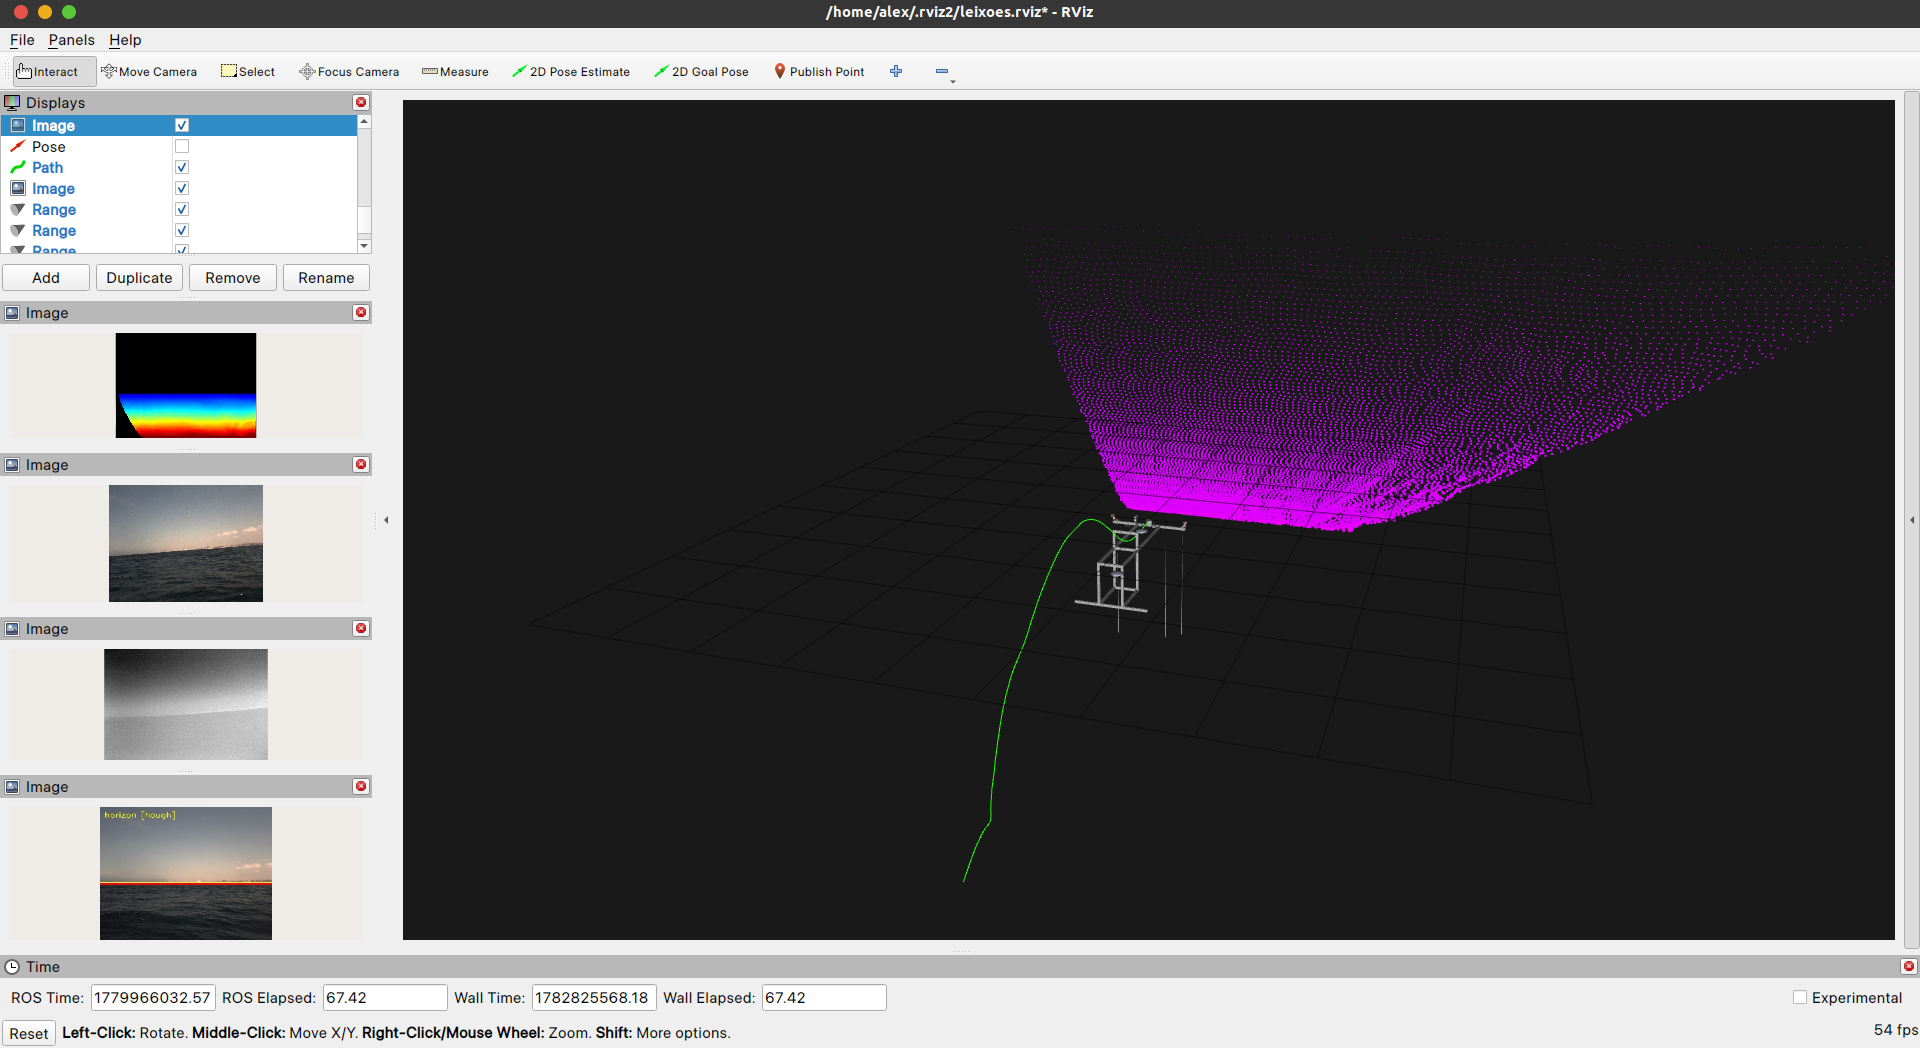
\includegraphics[width=\textwidth]{full_rviz}
    \caption{RViz visualization of the running pipeline. The 3D viewport (right) shows the georeferenced sea-surface point cloud and the sensor rig wireframe, with the platform's travelled path (green) overlaid in the \texttt{map} (ENU) frame. The left panel shows live image feeds: the rainbow-coded disparity map, the rectified left camera image, the thermal camera, and the horizon-detection output with the sky-exclusion line marked in red.}
    \label{fig:rviz-screenshot}
\end{figure}

The sensor frame layout used by the visualization is shown in Figure~\ref{fig:tf-frame-tree}.


\subsection{Validation}

\label{sec:validation}

With no wave buoy or other ground truth available for this dataset, validation relied on cross-checking the two independent wave estimators against each other, and on cross-checking the navigation/altitude pipeline against an independent reference signal. Each of the cases below follows the same pattern: a method was applied, a measurement revealed a quantitatively implausible or inconsistent result, a specific cause was diagnosed from the raw data, a fix was applied, and the corrected result was re-checked. Consistent with the characterize, implement and re-verify process described in the Methodology.

\textbf{Altimeter spectrum noise floor.} The first live run of the altimeter-based wave estimator produced a significant wave height of $\approx$2.3~m at a peak period of $\approx$1.7~s, a combination that implies a wave steepness well past the physical breaking limit, and therefore not a real sea state. Comparing the altimeter's elevation spectrum against the navigation filter's own altitude spectrum over the same window showed that the altimeter range carries a broadband sensor-noise floor that does not roll off above the real wave-frequency peak; integrating over the full available frequency band (rather than just the wave band) picked up that noise and inflated the height estimate roughly fourfold. Band-limiting the spectral integration to the physically plausible wave-frequency range corrected this to $H_s\approx0.4$--0.6~m at $T_p\approx2$--2.4~s, which is the range used throughout the rest of the validation. The same comparison also showed that the navigation filter's altitude signal itself carries essentially no energy in the wave band (the platform does not measurably heave at wave frequencies on this dataset), so subtracting it from the raw range, the originally intended heave-compensation step, was disabled, since it only injected the navigation filter's own noise without removing any real heave. Figure~\ref{fig:altimeter-pipeline} shows the full altimeter processing pipeline, with the band-limiting step highlighted.

\begin{figure}[H]
	\centering
	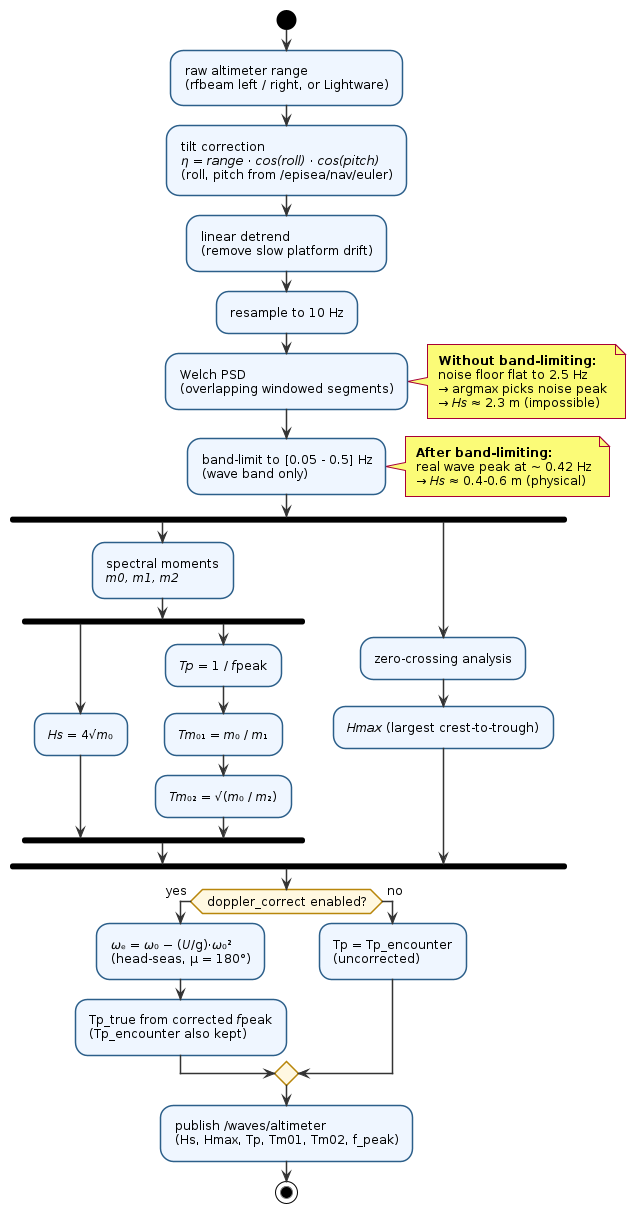
\includegraphics[width=0.72\textwidth,height=0.82\textheight,keepaspectratio]{diagrams/altimeter_wave_pipeline}
	\caption{Altimeter wave-estimation processing pipeline. The band-limiting step (highlighted) was the critical fix: integrating the full spectrum to Nyquist picked up the sensor noise floor and inflated $H_s$ roughly fourfold; restricting to the wave band [0.05--0.5~Hz] recovers the physical estimate.}
	\label{fig:altimeter-pipeline}
\end{figure}

\textbf{Point-cloud bad-frame contamination.} The point-cloud-based wave estimator initially produced an implausible maximum-wave-height estimate (2--9~m) at a significant height of only $\approx$0.5~m. Characterizing the surface-fit residuals frame by frame showed that roughly a third of frames suffered a whole-frame disparity failure (the entire reconstructed patch was spread out, not just a few stray points), so no single-frame outlier trimming could fix it. A per-frame quality gate was added that scores each frame's surface fit and discards the frame entirely if its implied wave height exceeds a physically reasonable threshold before it can contaminate the running estimate. This brought the height estimate down to a physically consistent value and improved the ratio between maximum and significant wave height from 4.6 (implausible) to 2.7 (consistent with real sea states). This per-frame quality gate is summarised in Figure~\ref{fig:bad-frame-gate}.

\begin{figure}[H]
	\centering
	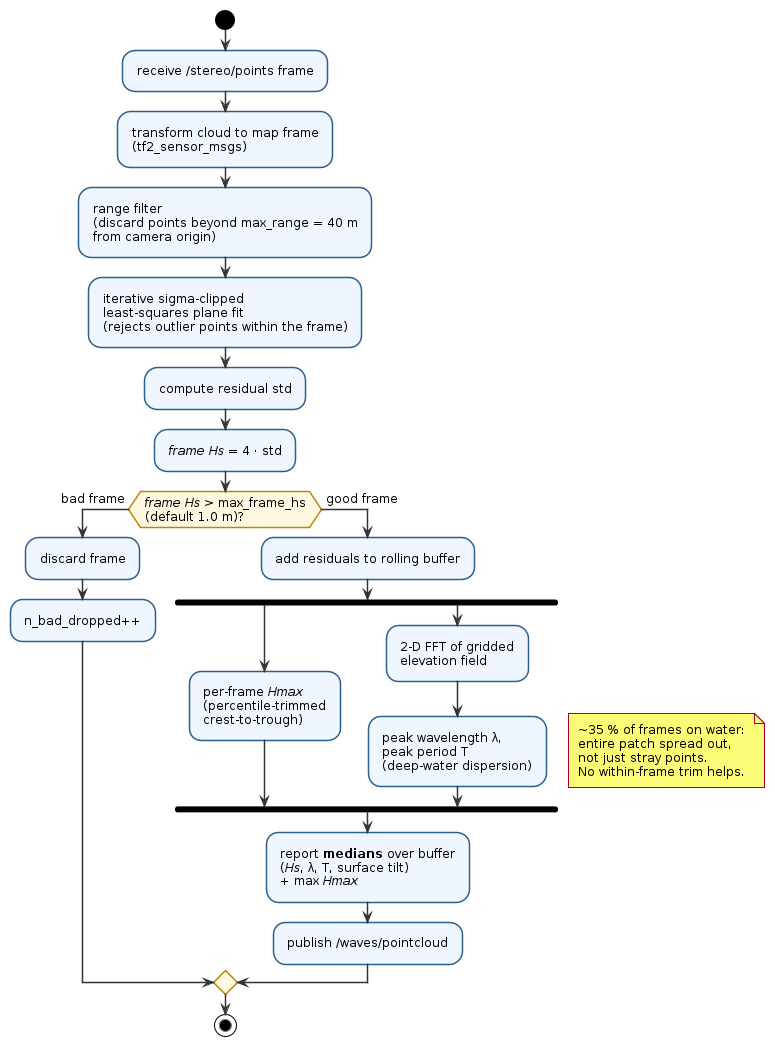
\includegraphics[width=0.72\textwidth,height=0.82\textheight,keepaspectratio]{diagrams/bad_frame_gate}
	\caption{Per-frame quality gate in the point-cloud wave estimator. Whole-frame disparity failures (affecting $\approx$35\% of frames on the water surface) spread the entire reconstructed patch; the gate drops these before they contaminate the running $H_s$ estimate.}
	\label{fig:bad-frame-gate}
\end{figure}

\textbf{Reconciling the point-cloud height with the altimeter.} Even after the bad-frame fix, the point-cloud height estimate read roughly half the altimeter's. This was traced to the imaging geometry rather than a remaining bug: the reconstructed patch spans a long, oblique range, and far points carry disproportionately large stereo error, which both inflates a purely vertical variance estimate and biases a tilted-plane fit (which partly absorbs real long-wavelength elevation as ``tilt''). Restricting the analysis to the near field, and reporting the median rather than the mean over the buffered frames (the bad-frame gate otherwise biases the mean down asymmetrically), brought the point-cloud height estimate into agreement with the altimeter's at the same instant in the recording.

\textbf{Reconciling the period estimate via a Doppler/en\-counter-fre\-quency correction.} Even with height reconciled, the altimeter's peak period ($\approx$2.1--2.4~s) and the point cloud's spatially derived period ($\approx$3.7~s) disagreed by far more than measurement noise could explain. Recognizing that this dataset was recorded from a moving boat platform (at $\approx$2.6~m/s, up to 3.8~m/s) rather than a stationary one explained the gap: the altimeter measures the wave \emph{encounter} period as seen by a moving observer, not the true period, while the spatial point-cloud estimate is motion-independent. Applying the standard deep-water encounter-to-true frequency correction (using the platform's own speed, under a head-seas assumption) converted the altimeter's encounter period to a true period of $\approx$3.2~s, in agreement with the point cloud's independent 3.7~s estimate to within $\approx$10--13\%. This single platform-speed correction resolved what had been the longest-standing disagreement between the two estimators, and is consistent with the role of platform motion in altimetric wave measurement reported for other moving platforms~\cite{ichikawa2024seasurface}. Figure~\ref{fig:doppler-correction} illustrates this encounter-to-true period correction.

\begin{figure}[H]
	\centering
	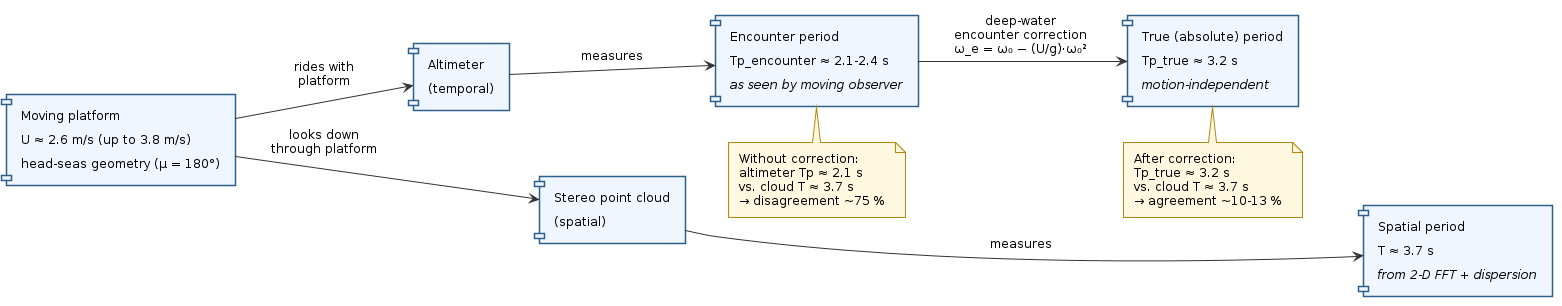
\includegraphics[width=\textwidth]{diagrams/doppler_correction}
	\caption{Doppler/encounter-frequency correction. The altimeter, riding with the moving platform, measures the encounter period; the stereo point cloud measures the spatial (true) period directly. Applying the deep-water encounter-to-true correction reduces the period disagreement from $\approx$75\% to $\approx$10--13\%.}
	\label{fig:doppler-correction}
\end{figure}

\textbf{Wave direction.} A least-squares fit of cross-spectrum phase across the three altimeters (arranged roughly along the boat's longitudinal axis) was used to estimate an off-axis angle relative to head seas. The fit is internally consistent within a single analysis window (sub-degree residual) and the cross-spectrum coherence is high, confirming the array senses a genuinely coherent wave, but the inferred angle is small relative to the array's short aperture and drifted noticeably (3--20\textdegree) across different windows as the boat manoeuvred. The array therefore confirms a roughly head-seas geometry and is reported as a diagnostic quantity, but was not considered reliable enough to override the head-seas assumption used in the Doppler correction above, nor to resolve a full heading (a single line of altimeters cannot distinguish port from starboard, or fore from aft). Wave direction is accordingly not delivered as a pipeline output; this is a known shortfall relative to the original proposal's directional objective, and resolving it would require either a 2-D sensor array with sufficient aperture relative to the dominant wavelength, or a different sensing modality altogether (e.g.\ the 2-D FFT over the stereo point cloud, which was implemented but dropped due to 180° ambiguity and near-random instability on this patch size -- see Section~\ref{sec:future}).

\textbf{Overall assessment.} The two wave-parameter estimators are independent in both sensing modality (temporal, single-point altimetry vs.\ spatial, multi-point stereo geometry) and failure mode, and after the corrections above they agree on significant wave height ($\approx$0.4--0.6~m) and on peak period ($\approx$3.2~s vs.\ 3.7~s) to within $\approx$10--13\%. This mutual agreement, achieved without any external ground truth, is the strongest evidence in this report that the pipeline's wave-parameter outputs are physically meaningful rather than artifacts of either sensing modality.


\section{Conclusions}

\subsection{Results achieved}

\label{sec:results}

The internship delivered a working, end-to-end ROS~2 pipeline that reconstructs a georeferenced 3D point cloud of the sea surface from a calibrated stereo pair and an independent navigation solution, and that extracts sea-state parameters from two independent sensing modalities. Against the objectives set out in Section~\ref{sec:objectives}: a working pipeline was built and demonstrated on real recorded data; six interchangeable disparity-estimation backends were implemented and systematically compared specifically to identify one that copes with the sea surface's low-texture, specular imaging conditions, which is the project's main technical contribution; and two independently derived, physically plausible wave estimates were obtained and cross-validated against each other without external ground truth, resolving along the way a series of unit, convention and noise-floor bugs that would otherwise have produced physically impossible results.

The pose/navigation estimate was likewise validated against an independent reference (the navigation filter's own modelled water level), with the resulting altitude residual converging to a small, stable value.

Relative to the original proposal, the modelling part of the work plan (state-of-the-art review, sensor characterization, estimation-algorithm development, validation) was completed and is the substance of this report; the wave-occurrence forecasting objective was descoped due to time-constraints in favour of consolidating reliable estimation first, and is carried forward as future work (Section~\ref{sec:future}).

\subsection{Lessons learned}

\label{sec:lessons}

The first lesson learned is that a literature-backed recommendation is a starting point, not a verdict: it has to be re-tested against the project's own data and constraints, because the conditions that made it the right answer in the source material do not automatically hold here. The disparity-backend comparison (Section~\ref{sec:architecture}) showed that a generic photometric-quality score, the kind of metric usually reported in the stereo-matching literature, was nearly uninformative between every backend that produced disparity at all, while an application-level signal (whether the downstream wave estimator could actually use the resulting point cloud, and how often it had to discard frames) was what actually separated the backends that solved the project's problem from those that did not. The literature pointed in a reasonable direction, but only testing in this project's specific context revealed whether it actually applied.

The second lesson is that fixing a result without understanding why it was wrong tends to produce another wrong result, just a less obviously wrong one. Several diagnoses in Section~\ref{sec:validation} only worked because the investigation went one level past ``the number looks bad'': the altimeter's implausible wave height was traced specifically to a broadband sensor-noise floor outside the wave band, not just patched by clamping the output, which is why band-limiting the spectral integration fixed it without also needing a heave correction that the noise floor had been masking. The same applies to the disparity comparison: StereoBM's apparent total failure under default parameters turned out to be a parameter-choice artifact rather than evidence that block matching cannot work on water at all, and SGM-CUDA's failure to ever support a usable point cloud was traced to the specific GPU binding lacking a left--right consistency control, not treated as a verdict on SGM in general.

The third lesson is that without a validation, comparison, or ground-truth signal, a result is just a number, with no way to tell whether it is measuring the real world or an artifact of the pipeline. No wave buoy or other ground truth was available for this dataset, so every claim in this report rests on cross-checking two estimators that fail in different, independent ways: a temporal, single-point altimeter signal against a spatial, multi-point stereo-geometry signal (Section~\ref{sec:validation}), and the navigation/altitude pipeline against the navigation filter's own modelled water level (Section~\ref{sec:results}). Every wave-estimation bug described in this report, the altimeter noise floor, the point-cloud bad-frame contamination, the height and period mismatches between the two estimators, was only caught because there were two independent numbers to disagree with each other in the first place; any one of them taken alone would have looked self-consistent and been wrong. That mutual agreement after the corrections, not either estimator individually, is what gives the project's wave-parameter outputs a more reliable meaning rather than just plausible-looking output.
\subsection{Future work}

\label{sec:future}

\begin{itemize}
	\item \textbf{Short-term wave-occurrence forecasting.} The original proposal's third phase: predicting near-future wave occurrence from the periodic structure already being extracted, using deterministic, statistical or learning-based methods, was descoped during this internship in favour of consolidating reliable parameter estimation first (Section~\ref{sec:objectives}). With two cross-validated estimators now in place, this is the natural next step.
	\item \textbf{Validation on a rougher sea state.} All validation in this report was performed on a single, comparatively calm recording. The heave-compensation step that was found unnecessary here, and the disparity-failure rate that is already $\approx$35\% before gating, should both be re-checked on a rougher-sea recording before generalizing the project's conclusions.
	\item \textbf{Validation on the intended airship platform.} This dataset was recorded from a boat, not the airship the project ultimately targets; the platform-motion assumptions used here (negligible heave, a head-seas Doppler correction) should be revisited once data from the actual WIG platform becomes available.
	\item \textbf{Validation against ground truth.} The two estimators were cross-validated against each other, but no independent ground truth was available for this dataset. A future test with a wave buoy array or a controlled wave tank would provide a more definitive validation of the pipeline's outputs.
	\item \textbf{Compilation of the WAFT-Stereo backend.} The WAFT-Stereo backend, which was the best performing disparity backend, was not compiled for the target embedded platform due to time constraints. A future step is to compile it for the Jetson Orin Nano using TensorRT or ONNX in order to improve the pipeline's latency.
\end{itemize}

\subsection{SDG impact}

This work contributes most directly to \textbf{SDG~13 (Climate Action)}: reliable, low-cost in-situ sea-state estimation supports ocean and climate monitoring, and is a building block for the kind of maritime environmental awareness that climate-adaptation and coastal-safety efforts depend on. It also contributes to \textbf{SDG~9 (Industry, Innovation and Infrastructure)}, by advancing the sensing infrastructure needed for a novel class of low-altitude, energy-efficient maritime aircraft (WIG vehicles), whose safe operation depends on exactly the kind of real-time sea-surface perception developed here. More broadly, accurate wave-parameter estimation from low-cost, multi-sensor platforms also has a direct bearing on maritime safety for any vessel or platform operating close to the sea surface, beyond the specific WIG use case that motivated this project.

\bibliographystyle{plain}
\bibliography{refs} % Entries are in the refs.bib file

\end{document}
